% 1-bit predictor state machine (matches rtl/one_bit_predictor.v)
% Build: cd docs/diagrams && tectonic one_bit_fsm.tex
\documentclass[tikz,border=6pt]{standalone}
\usetikzlibrary{arrows.meta,automata,positioning,calc}
\begin{document}
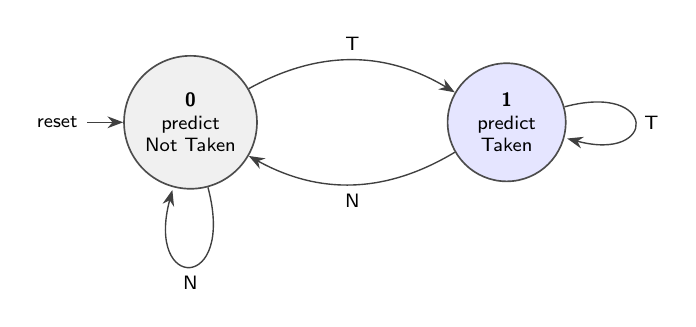
\begin{tikzpicture}[
  font=\sffamily\scriptsize, >={Stealth[length=2mm]}, node distance=24mm,
  st/.style={state, minimum size=15mm, align=center, draw=black!70, line width=0.6pt},
  every edge/.style={draw=black!75, line width=0.5pt}
]
\node[st, fill=black!6, initial, initial text={reset}] (s0) {\textbf{0}\\predict\\Not Taken};
\node[st, fill=blue!10, right=of s0] (s1) {\textbf{1}\\predict\\Taken};
\path[->]
  (s0) edge[bend left=30] node[above]{T} (s1)
  (s1) edge[bend left=30] node[below]{N} (s0)
  (s0) edge[loop below]   node[below]{N} (s0)
  (s1) edge[loop right]   node[right]{T} (s1);
\end{tikzpicture}
\end{document}
